\documentclass[aps,letterpaper,10pt]{article}

\usepackage{multirow}
\usepackage{graphicx} % For images
\usepackage{float}    % For tables and other floats
\usepackage{verbatim} % For comments and other
\usepackage{amsmath}  % For math
\usepackage{amssymb}  % For more math
\usepackage{fullpage} % Set margins and place page numbers at bottom center
\usepackage{listings} % For source code
\usepackage{subfigure}   % For subfigures
\usepackage[usenames,dvipsnames]{color} % For colors and names
\usepackage[pdftex]{hyperref}           % For hyperlinks and indexing the PDF
\usepackage{xcolor}

\hypersetup{ % play with the different link colors here
    colorlinks,
    citecolor=blue,
    filecolor=blue,
    linkcolor=blue,
    urlcolor=blue % set to black to prevent printing blue links
}


\lstdefinestyle{lfonts}{
basicstyle = \footnotesize\ttfamily,
stringstyle = \color{purple},
keywordstyle = \color{blue!60!black}\bfseries,
commentstyle = \rmfamily
}
\lstdefinestyle{lnumbers}{
numbers = left,
numberstyle = \tiny,
numbersep = 1em,
firstnumber = 1,
stepnumber = 1,
}
\lstdefinestyle{llayout}{
breaklines = true,
tabsize = 2,
columns = flexible,
}
\lstdefinestyle{lgeometry}{
xleftmargin = 20pt,
xrightmargin = 0pt,
frame = tb,
framesep = \fboxsep,
framexleftmargin = 20pt,
}
\lstdefinestyle{lgeneral}{
style = lfonts,
style = lnumbers,
style = llayout,
style = lgeometry,
}
\lstdefinestyle{python}{
language = {Python},
style = lgeneral,
}

\lstset{
    basicstyle          =   \sffamily,          % 基本代码风格
    keywordstyle        =   \bfseries,          % 关键字风格
    commentstyle        =   \rmfamily\itshape,  % 注释的风格,斜体
    stringstyle         =   \ttfamily,  % 字符串风格
    flexiblecolumns,                % 别问为什么,加上这个
    numbers             =   left,   % 行号的位置在左边
    showspaces          =   false,  % 是否显示空格,显示了有点乱,所以不现实了
    numberstyle         =   \zihao{-5}\ttfamily,    % 行号的样式,小五号,tt等宽字体
    showstringspaces    =   false,
    captionpos          =   t,      % 这段代码的名字所呈现的位置,t指的是top上面
    frame               =   lrtb,   % 显示边框
}



% Make units a little nicer looking and faster to type
\newcommand{\Hz}{\textsl{Hz}}
\newcommand{\KHz}{\textsl{KHz}}
\newcommand{\MHz}{\textsl{MHz}}
\newcommand{\GHz}{\textsl{GHz}}
\newcommand{\ns}{\textsl{ns}}
\newcommand{\ms}{\textsl{ms}}
\newcommand{\s}{\textsl{s}}
\newcommand{\RNum}[1]{\uppercase\expandafter{\romannumeral #1\relax}}


% TITLE PAGE CONTENT %%%%%%%%%%%%%%%%%%%%%%%%
% Remember to fill this section out for each
% lab write-up.
%%%%%%%%%%%%%%%%%%%%%%%%%%%%%%%%%%%%%%%%%%%%%
\newcommand{\labno}{05}
\newcommand{\labtitle}{AU 332 Artificial Intelligence: Principles and Techniques}
\newcommand{\authorname}{Zhengbao He(517030910157) \& Jingwei Zhao(5517030910047)}
\newcommand{\hw}{2}
% END TITLE PAGE CONTENT %%%%%%%%%%%%%%%%%%%%


\begin{document}  % START THE DOCUMENT!


% TITLE PAGE %%%%%%%%%%%%%%%%%%%%%%%%%%%%%%%%%%%%%%
% If you'd like to change the content of this,
% do it in the "TITLE PAGE CONTENT" directly above
% this message
%%%%%%%%%%%%%%%%%%%%%%%%%%%%%%%%%%%%%%%%%%%%%%%%%%%
\begin{titlepage}
\begin{center}
{\Large \textsc{\labtitle} \\ \vspace{4pt}}
\rule[13pt]{\textwidth}{1pt} \\ \vspace{150pt}
{\large By: \authorname \\ \vspace{10pt}
HW\#: \hw \\ \vspace{10pt}
\today}
\end{center}
\end{titlepage}
% END TITLE PAGE %%%%%%%%%%%%%%%%%%%%%%%%%%%%%%%%%%





%%%%%%%%%%%%%%%%%%%%%%%%%%%%%%
%%%%%%%%%%%%%%%%%%%%%%%%%%%%%%
\section{Introduction}
%No Text Here
%%%%%%%%%%%%%%%%%%%%%%%%%%%%%%%
\subsection{Purpose}
In this assignment, we are going to apply minimax search with alpha-beta pruning on Chinese Checkers, in the aim of building an intelligent Chinese Checkers play agent and winning the tournament.

Through this assignment, we will design and implement a Minimax algorithm 
and try to optimize it using alpha-beta pruning. Besides, we will devise a decent evaluation function as searching heuristics because we can not search the whole adversarial tree with limited computing resources.

Finishing this assignment, we are more conversant with the concept of adversarial search, as well as basic algorithms such as MiniMax and Alpha-Beta Pruning, and how to implement them.

\vspace{3mm} % I use this to seperate the paragraphs a bit.

%%%%%%%%%%%%%%%%%%%%%%%%%%%%%%
\subsection{Equipment}
	\begin{itemize}
		\item A laptop with Windows 10 or Linux
		\item Anaconda 3
		\item VS Code 
		\item TexLive
	\end{itemize}

\subsection{Procedure}
\begin{enumerate}
\item Implement Minimax and Alpha-Beta Pruning algorithms in python file {\itshape agent.py}.
\item Devise an evaluation function, which returns a heristic value indicating which step to take at a cetain searching depth. The evaluation function is necessary because we can not search the whole adversarial tree due to limited computing resources. 
\item Test the agent, refine the algorithms, and enhance the agent's performance.
\end{enumerate}

\newpage
\section{Code and algorithm}
This section will introduce the code and algorithm we design and some attempts we made.
\vspace{3mm}


% IF YOU'D RATHER TYPE THE CODE, OR HAVE A SMALLER BLOCK OF CODE, USE THIS:
%\begin{lstlisting}
%if(something)
%	do this
%else
%	do this
%\end{lstlisting}#print('\t'*depth + "第{}层节点生成,alpha = {},beta = {}".format(depth, alpha, beta))

%% THIS IS FROM A DIFFERENT CLASS, BUT DEMONSTRATES MATH MODE WELL
%%%%%%%%%%%%%%%%%%%%%%%%%%%%%%
\subsection{The basic Minimax algorithm with alpha-beta pruning}

The code below implements a simple MiniMax algorithm with alpha-beta pruning and the default depth is 2, which means that we only consider two movement of our pieces.
This is because when the pieces of both players are entangled, considering too many moves makes the algorithm very complicated. 
What we are thinking about is how to reach the end point faster than the opponent, and the opponent is also.
Because both players will give priority to their own movements, too deep search will introduce more uncertainty and consume more computing resources.
So when the two players’ pieces are not separated, we just use the MiniMax algorithm whose depth is 2.


\begin{lstlisting}[style = python]
def MiniMax_pruned_version(self, state, depth, al, be, Depth=2):
	if depth != Depth:
		alpha = al
		beta = be
		if depth % 2 == 0:  # max layer
			evaluation = -10000
		else:
			evaluation = 10000
		selected_action = None
		legal_actions = self.game.actions(state)
		player = state[0]
		for action in self.stimulation_max(state, legal_actions):
			if action[1][0]*(-1)**player < action[0][0]*(-1)**player:
				continue
			board = state[1]
			board.board_status[action[0]] = 0
			board.board_status[action[1]] = player
			value, next_action = self.MiniMax_pruned_version((3 - player, board), depth + 1, al=alpha, be=beta)
			board.board_status[action[0]] = player
			board.board_status[action[1]] = 0
			if depth % 2 == 0:  # max layer
				if value > evaluation:
					evaluation = value
					selected_action = action
					alpha = value
			else:  # min layer
				if value < evaluation:
					evaluation = value
					selected_action = action
					beta = value
			if alpha >= beta:
				#print('\t'*depth + "Pruned in layer",depth)
				return evaluation, selected_action
		return evaluation, selected_action
	else:
		evaluation_value = self.evaluation(state, p=2, i=10, d=5)
		return evaluation_value, None
\end{lstlisting}




\subsection{SelfMax algorithm}
When two players’ pieces are separated, we apply another algorithm which we refer to as {\itshape SelfMax} algorithm.
It just considers the movement of the agent itself, without considering that of the opponent.
So in this case, since pieces of two players have already been saparated with each side, movement of each side will not affect the other. 
Thus considering opponent's movement only consume computing resources.
Bacause we don't need to consider the opponent's movement, the two factors limiting depth in MiniMax above disappear, we can deepen the search depth and get better performence.
The detailed codes of {\itshape SelfMax} are listed below(the variable {\itshape Depth} is 2 means that we consider 3 movements of our agent).

\begin{lstlisting}[style=python]
def selfMax(self, state, depth, Depth=2):
	if depth != Depth:
		evaluation = -10000
		selected_action = None
		legal_actions = self.game.actions(state)
		player = state[0]
		for action in self.stimulation_max(state, legal_actions):
			if action[1][0] * (-1) ** player < action[0][0] * (-1) ** player:
				continue
			board = state[1]
			board.board_status[action[0]] = 0
			board.board_status[action[1]] = player
			ver_positions = [position[0] for position in board.getPlayerPiecePositions(player)]
			if sum(ver_positions) == (2 - player) * 30 + (player - 1) * 170:
				board.board_status[action[0]] = player
				board.board_status[action[1]] = 0
				return 10000, action
			value, next_action = self.selfMax((player, board), depth + 1)
			board.board_status[action[0]] = player
			board.board_status[action[1]] = 0
			if value > evaluation:
				evaluation = value
				selected_action = action
		return evaluation, selected_action
	else:
		evaluation = self.evaluation(state, p=1, i=5, d=0)
		return evaluation, None
\end{lstlisting}



\subsection{Evaluation Function}
When the search depth is limited because of limited computing resources, it is very important to evaluate the current game when the outcome is not divided.
In the evaluation function below, we use four factors to evaluate the move decision:
\begin{itemize}
\item Total vertical distancement of our pieces
\item The distance of the piece from the center line of the board
\item The lagger piece--the piece at the end of the board
\item Total vertical distancement of opponent's pieces
\end{itemize}

We use three parameters {\itshape p}, {\itshape i}, and {\itshape d} to weight the four different parts, where the total vertical distancement of our pieces and that of the opponent's pieces share the same parameter ({\itshape p}).

\begin{lstlisting}[style = python]
def evaluation(self, state, p, i, d):
	player = state[0]
	board = state[1]

	if player == 1:
		ver_positions = [position[0] for position in board.getPlayerPiecePositions(player)]
		op_p = [position[0] for position in board.getPlayerPiecePositions(3 - player)]
		hor_positions = [abs(position[1] - board.getColNum(position[0]) / 2) / board.getColNum(position[0]) for
							position in board.getPlayerPiecePositions(player) if position[0] % 2 == 0]

		ver_displacement = sum(ver_positions)
		lagger = 2 * board.size - 1 - max(ver_positions)
		hor_displacement = sum(hor_positions)
	else:
		ver_positions = [2 * board.size - 1 - position[0] for position in board.getPlayerPiecePositions(player)]
		op_p = [2 * board.size - 1 - position[0] for position in board.getPlayerPiecePositions(3 - player)]
		hor_positions = [abs(position[1] - board.getColNum(position[0]) / 2) / board.getColNum(position[0]) for
							position in board.getPlayerPiecePositions(player) if position[0] % 2 == 0]
		ver_displacement = sum(ver_positions)
		lagger = 2 * board.size - 1 - max(ver_positions)
		hor_displacement = sum(hor_positions)

	return - p * ver_displacement + i * lagger - d * hor_displacement - p * sum(op_p)
\end{lstlisting}

It's obvious that we should use the total vertical distance to evaluate the game because a smaller vertical distance means more possiblility to win.
And it's also better to stay close to the center line of the board. 
When a piece is on the edge of the board, it has less chances to interact with other pieces,
which means less possiblity to make a long hop.
We also consider the "lagger" piece. If one piece is left behind by other pieces, it's more likely to move step by step.
The last factor we consider is the total vertical distance of opponent's pieces. 
The reason is that our opponent gives priority to his own movement. 
If we don't consider our opponent, the "MIN" in MiniMax is meaningless.

\section{Test and Performance}
In order to test the validity of our play agent, we make a series of testing games in which our agent competes with a greedy agent. The greedy agent tries to maximize its utility at each move. During the competition, we also modify the parameters of the evaluation funciton so as to let our agent more powerful. We finaly set the parameters {\itshape p}, {\itshape i}, and {\itshape d} to be 2, 10, and 5 respectively before pieces of two players are saparated with each other, and to be 1, 5, 0 after. 

The detailed competing results are show in figure, in which we can see our agent has absolute advantage over the greedy agent, since it wins all of the 100 sequential games which it takes the first step. When our agent takes the second step, it appears to be less advantageous than the previous situation, but it still shows much more superiority to the greedy agent, with 98 wins and 2 ties in a sequence of 100 games.

\begin{figure}[!h] \centering    
	\subfigure[Our agent takes the first step] {
		\label{first}     
	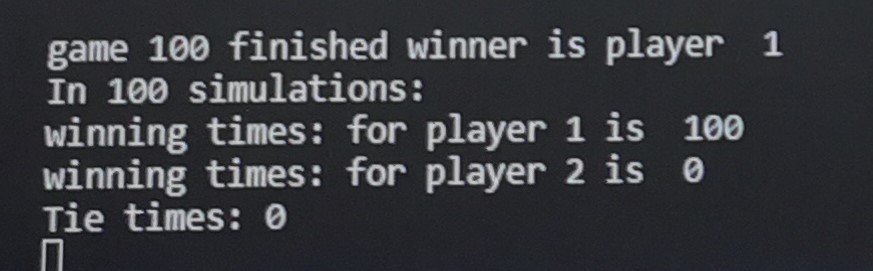
\includegraphics[width=0.45\columnwidth]{first.jpg}
	}     
	\subfigure[Our agent takes the second step] { 
	\label{second}     
	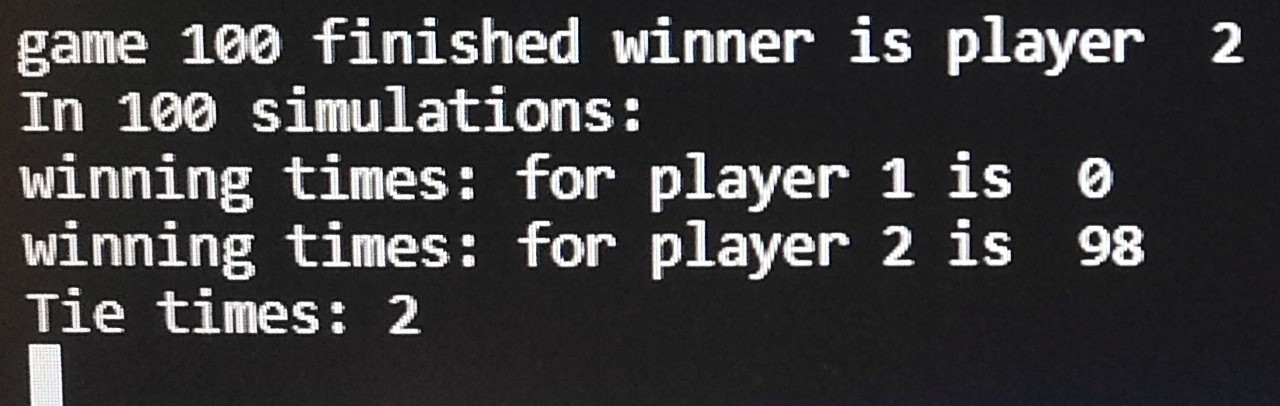
\includegraphics[width=0.45\columnwidth]{second.jpg}     
	}    
	\caption{ Results of simulation games with a greedy agent }     
	\label{games}     
\end{figure} 
%%%%%%%%%%%%%%%%%%%%%%%%%%%%%%
\newpage
\section{Discussion \& Conclusion}
In this assignment, we implemented an inteligent agent pleyer to play Chinese Checkers. Concretely, we assume both players are intelligent enough, and utilize depth limited MiniMax algorithm to select a next step. In order to enhance time efficiency, we further implemented alpha-beta pruning so that the MiniMax algorithm can go down deeper through the adversarial tree. 

On innovation of our design is that, we realise that it is not reasonable to continue with MiniMax algorithm after the pieces of both players saparate with each side. At this moment, both sides will no longer interact with each other, thus we do not have to consider the opponent's movement. As a result, our agent only goes down the tree to maxmize its own utility. In practice, our disign effectively booms the performance of our agent.
\end{document} % DONE WITH DOCUMENT!


